% ---------------------------------------------------------------------------
%  Lecture notes -- Lab S2: Influence Lines (UTM Civil Engineering Laboratory II)
%  Build: xelatex s2_lecture_notes.tex  (twice)
% ---------------------------------------------------------------------------
\documentclass[11pt,a4paper]{article}
\usepackage{iftex}
\ifPDFTeX\usepackage[utf8]{inputenc}\usepackage[T1]{fontenc}\usepackage{lmodern}\else
\usepackage{fontspec}\usepackage{unicode-math}\setmainfont{Latin Modern Roman}\setsansfont{Latin Modern Sans}\setmathfont{Latin Modern Math}\fi
\usepackage[a4paper,margin=24mm,headheight=14pt]{geometry}
\usepackage{amsmath,mathtools,booktabs,array,multirow,siunitx,graphicx,xcolor,enumitem,caption,fancyhdr,tikz,tcolorbox,microtype}
\usepackage[hidelinks]{hyperref}
\tcbuselibrary{skins,breakable}
\graphicspath{{../figures/}}
% ---------------------------------------------------------------------------
%  s2figs.tex -- shared TikZ drawings for Lab S2 (Influence Lines)
%  Geometry in mm: A=0, B=250, C=440, D=690, E=880, F=1130.
%  \ILscale (cm per mm) is set by the including document before use.
% ---------------------------------------------------------------------------
\usetikzlibrary{arrows.meta,calc,patterns,decorations.pathreplacing}
\providecommand{\ILscale}{0.0115}
\colorlet{s2load}{orange!80!black}
\colorlet{s2reac}{blue!65!black}
\colorlet{s2hinge}{violet!80!black}
\colorlet{s2neg}{red!75!black}

% support symbols (anchored at beam centre line)
% offsets are given in cm so that the symbols keep their size whatever the x scale
\newcommand{\ILpin}[1]{%
  \draw[thick] (#1,-0.08) -- ++(-0.18cm,-0.3cm) -- ++(0.36cm,0) -- cycle;
  \draw[thick] ($(#1,-0.39)+(-0.26cm,0)$) -- ++(0.52cm,0);
  \foreach \t in {-0.22,-0.11,0,0.11,0.22} \draw ($(#1,-0.39)+(\t cm,0)$) -- ++(-0.08cm,-0.1cm);}
\newcommand{\ILroller}[1]{%
  \draw[thick] (#1,-0.08) -- ++(-0.18cm,-0.3cm) -- ++(0.36cm,0) -- cycle;
  \draw[thick] ($(#1,-0.45)+(-0.1cm,0)$) circle [radius=0.06cm] ($(#1,-0.45)+(0.1cm,0)$) circle [radius=0.06cm];
  \draw[thick] ($(#1,-0.52)+(-0.26cm,0)$) -- ++(0.52cm,0);
  \foreach \t in {-0.22,-0.11,0,0.11,0.22} \draw ($(#1,-0.52)+(\t cm,0)$) -- ++(-0.08cm,-0.1cm);}
\newcommand{\ILhingeat}[1]{\fill[white] (#1,0) circle [radius=0.11cm]; \draw[thick,s2hinge] (#1,0) circle [radius=0.11cm];}

% ---- the bridge model (elevation), with halts and span dimensions -----------
% optional argument: extra TikZ code drawn in the same picture (loads, arrows)
\newcommand{\ILbridge}[1][]{%
\begin{tikzpicture}[x=\ILscale cm,y=1cm,>=Stealth,font=\small]
  \pgfmathsetmacro{\xB}{250}\pgfmathsetmacro{\xC}{440}\pgfmathsetmacro{\xD}{690}\pgfmathsetmacro{\xE}{880}\pgfmathsetmacro{\xF}{1130}
  % beams
  \draw[line width=2.4pt] (0,0) -- (430,0);
  \draw[line width=2.4pt] (450,0) -- (680,0);
  \draw[line width=2.4pt] (700,0) -- (1130,0);
  \ILhingeat{440}\ILhingeat{690}
  \ILpin{0}\ILroller{250}\ILroller{880}\ILpin{1130}
  % halts
  \foreach \x/\l in {0/A,250/B,440/C,690/D,880/E,1130/F}
    \node[below,font=\small\bfseries] at (\x,-0.62) {\l};
  \foreach \x/\l in {100/1,200/2,300/3,400/4,500/5,600/6,700/7,800/8,900/9,1000/10,1100/11}
    {\draw (\x,-0.05) -- (\x,-0.22); \node[below,font=\scriptsize] at (\x,-0.22) {\l};}
  % dimensions
  \draw[|<->|] (0,-1.15) -- (250,-1.15) node[midway,below,font=\scriptsize] {250};
  \draw[|<->|] (250,-1.15) -- (440,-1.15) node[midway,below,font=\scriptsize] {190};
  \draw[|<->|] (440,-1.15) -- (690,-1.15) node[midway,below,font=\scriptsize] {250};
  \draw[|<->|] (690,-1.15) -- (880,-1.15) node[midway,below,font=\scriptsize] {190};
  \draw[|<->|] (880,-1.15) -- (1130,-1.15) node[midway,below,font=\scriptsize] {250};
  \node[font=\scriptsize,anchor=west] at (1140,-1.15) {mm};
  #1
\end{tikzpicture}}

% a downward load arrow at x (mm) with label
\newcommand{\ILload}[3][1.1]{\draw[->,very thick,s2load] (#2,#1) -- (#2,0.14) node[pos=0,above,font=\small\bfseries,s2load] {#3};}
% an upward reaction arrow at x with label (positive); negative drawn downward in red
\newcommand{\ILreaction}[3][0.9]{\draw[->,very thick,s2reac] (#2,-0.95-#1) -- (#2,-0.72) node[pos=0,below,font=\small,s2reac] {#3};}
\newcommand{\ILreactionneg}[3][0.9]{\draw[->,very thick,s2neg] (#2,-0.72) -- (#2,-0.95-#1) node[below,font=\small,s2neg] {#3};}

% ---- influence line plot: #1 = reaction name, #2 = list of x/y vertices -----
% #3 (optional) extra code; ordinate scale 1 unit = \ILyscale cm
\providecommand{\ILyscale}{1.0}
\newcommand{\ILilplot}[3][]{%
\begin{tikzpicture}[x=\ILscale cm,y=\ILyscale cm,>=Stealth,font=\small]
  \draw[gray!50,dashed] (250,-0.95) -- (250,1.95) (440,-0.95) -- (440,1.95) (690,-0.95) -- (690,1.95) (880,-0.95) -- (880,1.95);
  \draw[->] (0,0) -- (1180,0) node[right,font=\scriptsize] {$x$ (mm)};
  \foreach \x/\l in {0/A,250/B,440/C,690/D,880/E,1130/F} \node[below,font=\scriptsize\bfseries] at (\x,-0.02) {\l};
  \draw[very thick,s2reac] plot coordinates {#3};
  \node[anchor=south west,font=\small] at (0,1.5) {IL for #2};
  #1
\end{tikzpicture}}

% generated by s2_numbers.py / table script -- do not edit by hand
\newcommand{\TabOrdinates}{%
A & 0 & 1.000 & 0.000 & 0.000 & 0.000 & 0.000 & 0.000\\
1 & 100 & 0.600 & 0.400 & 0.000 & 0.000 & 0.000 & 0.000\\
2 & 200 & 0.200 & 0.800 & 0.000 & 0.000 & 0.000 & 0.000\\
B & 250 & 0.000 & 1.000 & 0.000 & 0.000 & 0.000 & 0.000\\
3 & 300 & -0.200 & 1.200 & 0.000 & 0.000 & 0.000 & 0.000\\
4 & 400 & -0.600 & 1.600 & 0.000 & 0.000 & 0.000 & 0.000\\
C & 440 & -0.760 & 1.760 & 1.000 & 0.000 & 0.000 & 0.000\\
5 & 500 & -0.578 & 1.338 & 0.760 & 0.240 & 0.422 & -0.182\\
6 & 600 & -0.274 & 0.634 & 0.360 & 0.640 & 1.126 & -0.486\\
D & 690 & 0.000 & 0.000 & 0.000 & 1.000 & 1.760 & -0.760\\
7 & 700 & 0.000 & 0.000 & 0.000 & 0.000 & 1.720 & -0.720\\
8 & 800 & 0.000 & 0.000 & 0.000 & 0.000 & 1.320 & -0.320\\
E & 880 & 0.000 & 0.000 & 0.000 & 0.000 & 1.000 & 0.000\\
9 & 900 & 0.000 & 0.000 & 0.000 & 0.000 & 0.920 & 0.080\\
10 & 1000 & 0.000 & 0.000 & 0.000 & 0.000 & 0.520 & 0.480\\
11 & 1100 & 0.000 & 0.000 & 0.000 & 0.000 & 0.120 & 0.880\\
F & 1130 & 0.000 & 0.000 & 0.000 & 0.000 & 0.000 & 1.000\\
}
\newcommand{\TabCompound}{%
A & 0 & 100 & 6.50 & 1.00\\
1 & 100 & 200 & 3.50 & 4.00\\
2 & 200 & 300 & 0.50 & 7.00\\
B & 250 & 350 & -1.00 & 8.50\\
3 & 300 & 400 & -2.50 & 10.00\\
4 & 400 & 500 & -4.44 & 11.34\\
C & 440 & 540 & -4.94 & 11.44\\
5 & 500 & 600 & -3.57 & 8.27\\
6 & 600 & 700 & -1.37 & 3.17\\
D & 690 & 790 & 0.00 & 0.00\\
}
\newcommand{\TabPracticeStudent}{%
A & 0 & 51 & & & \\
1 & 100 & 29 & & & \\
2 & 200 & 10 & & & \\
B & 250 & 1 & & & \\
3 & 300 & -11 & & & \\
4 & 400 & -28 & & & \\
C & 440 & -39 & & & \\
5 & 500 & -29 & & & \\
6 & 600 & -13 & & & \\
D & 690 & -1 & & & \\
7 & 700 & 0 & & & \\
8 & 800 & 0 & & & \\
E & 880 & 1 & & & \\
9 & 900 & -1 & & & \\
10 & 1000 & 0 & & & \\
11 & 1100 & 1 & & & \\
F & 1130 & 0 & & & \\
}
\newcommand{\TabPracticeKey}{%
A & 0 & 51 & 1.020 & 1.000 & +0.020 & +2.0\\
1 & 100 & 29 & 0.580 & 0.600 & -0.020 & -3.3\\
2 & 200 & 10 & 0.200 & 0.200 & 0.000 & +0.0\\
B & 250 & 1 & 0.020 & 0.000 & +0.020 & --\\
3 & 300 & -11 & -0.220 & -0.200 & -0.020 & -10.0\\
4 & 400 & -28 & -0.560 & -0.600 & +0.040 & +6.7\\
C & 440 & -39 & -0.780 & -0.760 & -0.020 & -2.6\\
5 & 500 & -29 & -0.580 & -0.578 & -0.002 & -0.3\\
6 & 600 & -13 & -0.260 & -0.274 & +0.014 & +5.1\\
D & 690 & -1 & -0.020 & 0.000 & -0.020 & --\\
7 & 700 & 0 & 0.000 & 0.000 & 0.000 & --\\
8 & 800 & 0 & 0.000 & 0.000 & 0.000 & --\\
E & 880 & 1 & 0.020 & 0.000 & +0.020 & --\\
9 & 900 & -1 & -0.020 & 0.000 & -0.020 & --\\
10 & 1000 & 0 & 0.000 & 0.000 & 0.000 & --\\
11 & 1100 & 1 & 0.020 & 0.000 & +0.020 & --\\
F & 1130 & 0 & 0.000 & 0.000 & 0.000 & --\\
}

\renewcommand{\ILscale}{0.0118}
\sisetup{per-mode=symbol}
\captionsetup{font=small,labelfont=bf,skip=4pt}
\setlist{nosep,leftmargin=*,itemsep=2pt}
\setlength{\parindent}{0pt}\setlength{\parskip}{5pt plus 1pt}
\pagestyle{fancy}\fancyhf{}
\fancyhead[L]{\small\itshape SEAA 3012 Civil Engineering Laboratory II}\fancyhead[R]{\small\itshape Lab S2 -- Influence Lines}
\fancyfoot[C]{\small\thepage}
\newtcolorbox{keybox}[1][]{enhanced,colback=blue!4,colframe=blue!55!black,fonttitle=\bfseries,title={#1},left=5pt,right=5pt,top=4pt,bottom=4pt,arc=2pt,boxrule=0.6pt}
\newtcolorbox{stepbox}[1][]{enhanced,breakable,colback=white,colframe=black!55,fonttitle=\bfseries,title={#1},left=5pt,right=5pt,top=4pt,bottom=4pt,arc=1.5pt,boxrule=0.5pt}
\newtcolorbox{activitybox}[1][]{enhanced,colback=orange!6,colframe=orange!75!black,fonttitle=\bfseries,title={#1},left=5pt,right=5pt,top=4pt,bottom=4pt,arc=2pt,boxrule=0.6pt}



\newcommand{\il}[1]{\eta_{#1}}

\title{\vspace{-14mm}\textbf{Lecture Notes: Influence Lines}\\[3pt]\large Lab S2 -- Cantilever (Gerber) Bridge Model}
\author{SEAA 3012 Civil Engineering Laboratory II\\Faculty of Civil Engineering, Universiti Teknologi Malaysia}
\date{Revised edition, 2026}

\begin{document}
\maketitle
\thispagestyle{fancy}

\section*{Learning outcomes}
After this session and the laboratory you should be able to
\begin{enumerate}
  \item define an influence line and distinguish it from a shear-force or bending-moment diagram;
  \item derive, by statics alone, the influence lines for the support reactions and hinge forces of the laboratory bridge model;
  \item use the Müller--Breslau principle to sketch and check an influence line;
  \item use an influence line to find the effect of a single load, a series of loads and a uniformly distributed load, and to locate the critical load position;
  \item reduce the dial-gauge readings of the experiment to experimental ordinates, compare them with theory and explain the discrepancies (CLO2, CLO4).
\end{enumerate}

\section{Why influence lines?}
Most structures are designed for loads that stay where they are: the weight of a floor, the water in a tank. A bridge, a crane girder or a gantry rail carries loads that \emph{move}, and the designer must answer a question that a shear-force diagram cannot: \emph{where} must the vehicle stand to produce the largest reaction at a pier, the largest shear at a section, or the largest moment at midspan? The influence line answers it directly.

\begin{keybox}[Definition]
The \textbf{influence line} (IL) of a response quantity $R$ (a reaction, a shear force, a bending moment, a deflection) at a \emph{fixed} point of a structure is the graph of that quantity against the position $x$ of a \emph{unit} concentrated load moving across the structure. Its ordinate is written $\il{R}(x)$ and has the units of $R$ per unit load (dimensionless for a reaction).
\end{keybox}

The contrast with the familiar diagrams is worth stating once and remembering (Table~\ref{tab:contrast}).

\begin{table}[h]
\centering\small
\caption{Influence line versus shear-force or bending-moment diagram.}
\label{tab:contrast}
\begin{tabular}{@{}p{3.6cm}p{5.3cm}p{5.3cm}@{}}
\toprule
 & Shear-force / bending-moment diagram & Influence line\\
\midrule
What is fixed & the loads & the point (section, support) where $R$ is evaluated\\
What varies along the abscissa & the section where $V$ or $M$ is read & the position $x$ of the unit load\\
What the ordinate means & $V$ or $M$ at that section, for the given loads & $R$ at the fixed point, for a unit load standing at $x$\\
\bottomrule
\end{tabular}
\end{table}

For a linear elastic structure the response is proportional to the load and the effects of several loads add (superposition), which is what makes the influence line useful: once $\il{R}(x)$ is known for a unit load, the effect of \emph{any} pattern of concentrated or distributed loads follows by multiplication and addition (Section~\ref{sec:use}).

\section{The laboratory model}
\label{sec:model}
The model in the Structures Laboratory (Figure~\ref{fig:model}) is a cantilever bridge of the type patented by Heinrich Gerber in 1866 and used, at a very different scale, in the Forth Bridge: two anchor spans with cantilever arms, and a \emph{suspended span} that simply rests on the tips of the arms through hinges.

\begin{figure}[h]
\centering
\ILbridge
\caption{Elevation of the model. Supports A and F are pins, B and E are rollers; C and D are the hinges of the suspended span CD; 1--11 are the halts at which the mass is placed. Dial gauges under A, B, E and F read the support reactions; those under C and D read the hinge forces.}
\label{fig:model}
\end{figure}

\paragraph{Members.} Beam ABC is simply supported at A and B with a cantilever BC of \SI{190}{mm}. Beam DEF is its mirror image. The suspended span CD (\SI{250}{mm}) rests on the cantilever tips: the hinges at C and D transmit a vertical force but no bending moment.

\paragraph{Supports and hinges.} A support or a joint is described by what it \emph{stops}: every movement it prevents produces a force (or moment) in that direction, and every movement it allows produces none.

\begin{center}\small
\begin{tabular}{@{}llll@{}}\toprule
Restraint & Where & Transmits & Allows\\\midrule
Pin & A, F & vertical and horizontal force & rotation\\
Roller & B, E & vertical force only & rotation and horizontal movement\\
Hinge (internal) & C, D & force between the two members it joins & relative rotation, so $M = 0$ there\\\bottomrule
\end{tabular}
\end{center}
A hinge is not a support: it joins two members and passes a force from one to the other, but no bending moment. Each hinge therefore adds one equation, $M = 0$ at that point, which is what makes the model statically determinate. In the model the supports at A and F can also pull downwards, and their gauges register uplift as a negative reading.

\paragraph{Determinacy.} No horizontal load is applied, so the pins at A and F provide no horizontal reaction and there are four unknown vertical reactions, $R_A$, $R_B$, $R_E$, $R_F$. Plane statics gives two useful equations for the whole structure ($\sum F_y = 0$ and $\sum M = 0$), and each internal hinge supplies one more ($M = 0$ at C and at D): four equations for four unknowns. The structure is \textbf{statically determinate}, and every influence line in these notes follows from equilibrium alone, with no need for $EI$. That is also why every influence line turns out to be made of straight segments.

\paragraph{Sign convention.} Support reactions are positive upwards. The hinge forces $R_C$ and $R_D$ are the forces that the suspended span presses on the cantilever tips (positive downwards on the tip); they are what the gauges at C and D register. Positions are measured from A, $0 \le x \le \SI{1130}{mm}$.

\section{Derivation of the influence lines}
\label{sec:derive}
The whole derivation uses one idea three times: \emph{take moments about a support}. The order matters: the suspended span is analysed first, because it is the only member whose loads reach the others.

\begin{figure}[h]
\centering
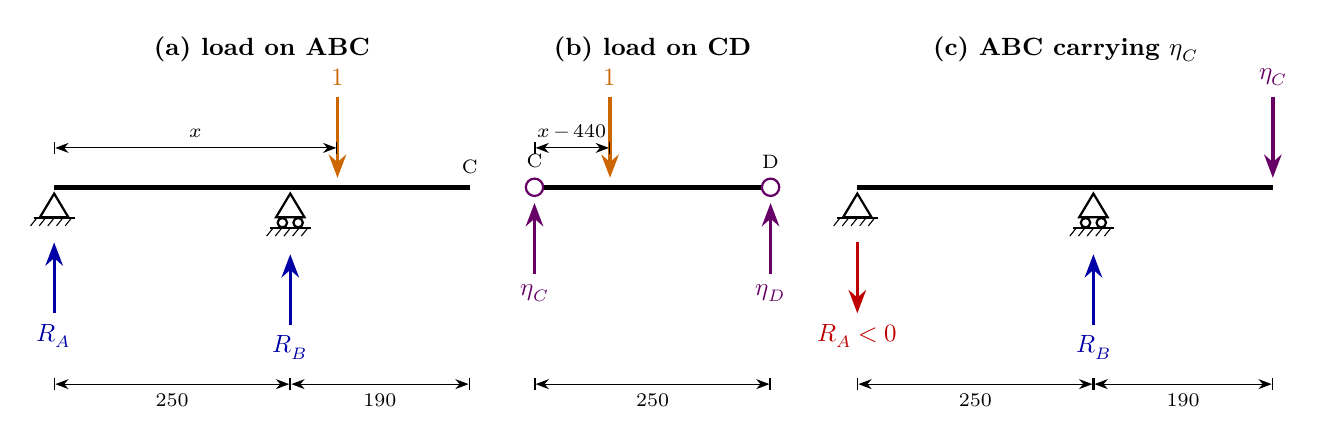
\begin{tikzpicture}[x=0.012cm,y=1cm,>=Stealth,font=\small]
  % (a) ABC with load
  \begin{scope}
    \draw[line width=2pt] (0,0) -- (440,0);
    \ILpin{0}\ILroller{250}
    \draw[->,very thick,s2load] (300,1.15) -- (300,0.12) node[pos=0,above,s2load] {$1$};
    \draw[->,very thick,s2reac] (0,-1.6) -- (0,-0.7) node[pos=0,below,s2reac] {$R_A$};
    \draw[->,very thick,s2reac] (250,-1.75) -- (250,-0.85) node[pos=0,below,s2reac] {$R_B$};
    \draw[|<->|] (0,0.5) -- (300,0.5) node[midway,above,font=\scriptsize] {$x$};
    \draw[|<->|] (250,-2.5) -- (440,-2.5) node[midway,below,font=\scriptsize] {190};
    \draw[|<->|] (0,-2.5) -- (250,-2.5) node[midway,below,font=\scriptsize] {250};
    \node[font=\small\bfseries] at (220,1.75) {(a) load on ABC};
    \node[above,font=\scriptsize] at (440,0.05) {C};
  \end{scope}
  % (b) suspended span
  \begin{scope}[xshift=6.1cm]
    \draw[line width=2pt] (0,0) -- (250,0);
    \ILhingeat{0}\ILhingeat{250}
    \node[above,font=\scriptsize] at (0,0.12) {C}; \node[above,font=\scriptsize] at (250,0.12) {D};
    \draw[->,very thick,s2load] (80,1.15) -- (80,0.12) node[pos=0,above,s2load] {$1$};
    \draw[->,very thick,s2hinge] (0,-1.1) -- (0,-0.2) node[pos=0,below,s2hinge] {$\il{C}$};
    \draw[->,very thick,s2hinge] (250,-1.1) -- (250,-0.2) node[pos=0,below,s2hinge] {$\il{D}$};
    \draw[|<->|] (0,0.5) -- (80,0.5) node[midway,above,font=\scriptsize] {$x-440$};
    \draw[|<->|] (0,-2.5) -- (250,-2.5) node[midway,below,font=\scriptsize] {250};
    \node[font=\small\bfseries] at (125,1.75) {(b) load on CD};
  \end{scope}
  % (c) ABC loaded by hinge force
  \begin{scope}[xshift=10.2cm]
    \draw[line width=2pt] (0,0) -- (440,0);
    \ILpin{0}\ILroller{250}
    \draw[->,very thick,s2hinge] (440,1.15) -- (440,0.12) node[pos=0,above,s2hinge] {$\il{C}$};
    \draw[->,very thick,s2neg] (0,-0.7) -- (0,-1.6) node[below,s2neg] {$R_A<0$};
    \draw[->,very thick,s2reac] (250,-1.75) -- (250,-0.85) node[pos=0,below,s2reac] {$R_B$};
    \draw[|<->|] (0,-2.5) -- (250,-2.5) node[midway,below,font=\scriptsize] {250};
    \draw[|<->|] (250,-2.5) -- (440,-2.5) node[midway,below,font=\scriptsize] {190};
    \node[font=\small\bfseries] at (220,1.75) {(c) ABC carrying $\il{C}$};
  \end{scope}
\end{tikzpicture}
\caption{Free-body diagrams used in Steps 1--3. In (c) the pull-down at A is drawn in the direction it actually acts.}
\label{fig:fbd}
\end{figure}

\begin{stepbox}[Step 1 -- Unit load on beam ABC ($0 \le x \le 440$)]
Isolate ABC (Figure~\ref{fig:fbd}a). It carries the unit load at $x$ and the two reactions $R_A$ and $R_B$; the hinge at C is unloaded because the suspended span carries nothing. Taking moments about B (anticlockwise positive),
\begin{equation}
  R_A \cdot 250 - 1\cdot(250 - x) = 0 \quad\Longrightarrow\quad
  \il{A}(x) = \frac{250 - x}{250},
  \label{eq:etaA1}
\end{equation}
and vertical equilibrium gives
\begin{equation}
  \il{B}(x) = 1 - \il{A}(x) = \frac{x}{250}.
  \label{eq:etaB1}
\end{equation}
Nothing in \eqref{eq:etaA1} stops at $x = 250$: for a load on the cantilever ($250 < x \le 440$) the lever arm $(250 - x)$ is negative, so $\il{A}$ is negative (the support at A must hold the beam down) and $\il{B}$ exceeds 1. At the tip, $\il{A}(440) = -190/250 = -0.76$ and $\il{B}(440) = 440/250 = 1.76$.
\end{stepbox}

\begin{stepbox}[Step 2 -- Unit load on the suspended span CD ($440 \le x \le 690$)]
Isolate CD (Figure~\ref{fig:fbd}b). It is a simply supported beam of span \SI{250}{mm} resting on the hinges, so the hinge forces follow the lever rule:
\begin{equation}
  \il{C}(x) = \frac{690 - x}{250}, \qquad \il{D}(x) = \frac{x - 440}{250}, \qquad \il{C} + \il{D} = 1.
  \label{eq:etaCD}
\end{equation}
\end{stepbox}

\begin{stepbox}[Step 3 -- Carry the hinge force into beam ABC]
With the load on CD, beam ABC carries only the downward force $\il{C}$ at its tip C (Figure~\ref{fig:fbd}c). This is Step 1 with the load $\il{C}$ standing at $x = 440$:
\begin{equation}
  \begin{aligned}
  \il{A}(x) &= \il{C}(x)\,\frac{250 - 440}{250} = -0.76\,\il{C}(x),\\
  \il{B}(x) &= \il{C}(x)\,\frac{440}{250} = 1.76\,\il{C}(x),
  \end{aligned}
  \qquad 440 \le x \le 690.
  \label{eq:etaA2}
\end{equation}
At C the two expressions for $\il{A}$ agree ($-0.76$), so the influence line is continuous; at D, $\il{C} = 0$ and therefore $\il{A} = \il{B} = 0$.
\end{stepbox}

\begin{stepbox}[Step 4 -- Unit load on beam DEF ($690 \le x \le 1130$)]
Beam DEF is the mirror image of ABC about the centre of the model ($x = 565$), with E playing the part of B and F that of A. Reading the geometry from F,
\begin{equation}
  \il{F}(x) = \frac{x - 880}{250}, \qquad \il{E}(x) = \frac{1130 - x}{250}, \qquad 690 \le x \le 1130,
  \label{eq:etaEF}
\end{equation}
while for a load on CD the hinge force $\il{D}$ is carried by DEF exactly as $\il{C}$ was by ABC: $\il{E} = 1.76\,\il{D}$ and $\il{F} = -0.76\,\il{D}$. A load on ABC or on DEF never reaches the other side, because the suspended span is then unloaded and transmits nothing: $\il{A} = \il{B} = 0$ for $x \ge 690$, and $\il{E} = \il{F} = 0$ for $x \le 440$.
\end{stepbox}

\begin{stepbox}[Why $\il{C}$ and $\il{D}$ are non-zero only between C and D]
The gauge at C reads the force that passes through hinge C, from the suspended span into the tip of cantilever BC. A force can pass through the hinge only when the suspended span itself carries something.
\begin{itemize}[leftmargin=*,itemsep=2pt]
\item \emph{Load on ABC} ($x < 440$): ABC stands on its own supports A and B and takes the load to them directly. The suspended span carries nothing, so nothing passes through C: $\il{C} = 0$.
\item \emph{Load on CD} ($440 \le x \le 690$): CD is a simple beam between the two hinges, and each hinge takes its lever-rule share, $\il{C} = (690-x)/250$, from 1 at C to 0 at D.
\item \emph{Load on DEF} ($x > 690$): the mirror of the first case; the load goes to E and F, CD stays unloaded and $\il{C} = 0$.
\end{itemize}
\textbf{The jump at C.} Just left of C the load stands on the cantilever tip, which belongs to ABC, so it goes straight to A and B and $\il{C} = 0$; just right of C it stands on the suspended span at its support, so the whole load passes through the hinge and $\il{C} = 1$. The Müller--Breslau construction (Section~\ref{sec:mb}) gives the same picture: cut the vertical connection at C and lift the end of CD by 1 relative to the tip; ABC does not move, because A and B still support it, while CD rotates about D.
\end{stepbox}

\begin{stepbox}[Step 5 -- Assemble and check]
Table~\ref{tab:ordinates} lists the six ordinates at the seventeen halts and Figure~\ref{fig:ils} plots four of them. Three checks catch most mistakes:
\begin{enumerate}
  \item \emph{Equilibrium of the whole model:} $\il{A} + \il{B} + \il{E} + \il{F} = 1$ for every $x$ (the unit load must be carried by the four supports).
  \item \emph{Continuity at the hinges:} the two formulae for $\il{A}$ give the same value at C; likewise for $\il{B}$, $\il{E}$ and $\il{F}$ at C and D.
  \item \emph{Slopes:} on ABC the slope of $\il{A}$ is $-1/250$ per mm; on CD it is $+0.76/250$ per mm. A kink can only occur at a hinge (C, D), never at a support that lies within a rigid member (B).
\end{enumerate}
\end{stepbox}

\begin{table}[h]
\centering\small
\caption{Theoretical influence-line ordinates (per unit load) at the halts of the model.}
\label{tab:ordinates}
\begin{tabular}{@{}c r r r r r r r@{}}
\toprule
Halt & $x$ (mm) & $\il{A}$ & $\il{B}$ & $\il{C}$ & $\il{D}$ & $\il{E}$ & $\il{F}$\\
\midrule
\TabOrdinates
\bottomrule
\end{tabular}
\end{table}

\begin{figure}[p]
\centering
\renewcommand{\ILyscale}{0.95}
\ILilplot[{\node[s2reac,font=\scriptsize,above left] at (0,1) {1.00};\node[s2neg,font=\scriptsize,below] at (440,-0.76) {$-0.76$};}]{$R_A$}{(0,1) (250,0) (440,-0.76) (690,0) (1130,0)}\\[8pt]
\ILilplot[{\node[s2reac,font=\scriptsize,above] at (440,1.76) {1.76};\node[s2reac,font=\scriptsize,above left] at (250,1) {1.00};}]{$R_B$}{(0,0) (250,1) (440,1.76) (690,0) (1130,0)}\\[8pt]
\ILilplot[{\node[s2reac,font=\scriptsize,above] at (440,1) {1.00};}]{$R_C$ (hinge force)}{(0,0) (440,0) (440,1) (690,0) (1130,0)}\\[8pt]
\ILilplot[{\node[s2reac,font=\scriptsize,above] at (690,1.76) {1.76};\node[s2reac,font=\scriptsize,above right] at (880,1) {1.00};}]{$R_E$}{(0,0) (440,0) (690,1.76) (880,1) (1130,0)}
\caption{Influence lines for $R_A$, $R_B$, the hinge force $R_C$ and $R_E$ (ordinates to scale). $R_D$ and $R_F$ are the mirror images of $R_C$ and $R_A$ about $x = 565$~mm.}
\label{fig:ils}
\end{figure}

\section{The Müller--Breslau principle}
\label{sec:mb}
There is a faster way to obtain the \emph{shape} of an influence line, and it is the method practising engineers use to check a computer output.

\begin{keybox}[Müller--Breslau principle]
Remove the restraint corresponding to the response quantity $R$ and give the released structure a unit displacement in the direction of $R$ (unit translation for a reaction or shear, unit rotation for a moment). The deflected shape of the structure is the influence line of $R$.
\end{keybox}

For $R_A$: remove the support at A and lift that end by one unit. Beam ABC is rigid between the hinge and the support, so it rotates about B as a straight line: A rises by 1, and the tip C, \SI{190}{mm} on the other side of B, drops by $190/250 = 0.76$. The suspended span follows C and stays straight, so it drops linearly from $0.76$ at C to zero at D. Beam DEF is not disturbed at all. The result (Figure~\ref{fig:mb}) is exactly the influence line of Figure~\ref{fig:ils}, including the sign: where the structure moves \emph{against} the direction of the released reaction, the ordinate is negative.

\begin{figure}[h]
\centering
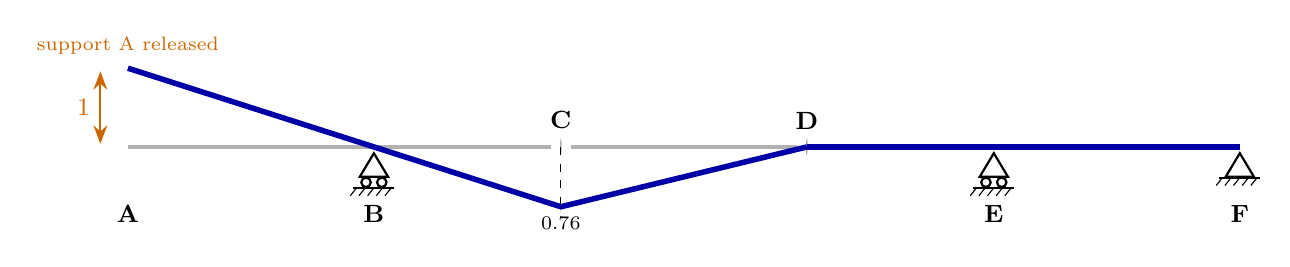
\begin{tikzpicture}[x=0.0125cm,y=1.0cm,>=Stealth,font=\small]
  \draw[gray!60,line width=1.6pt] (0,0) -- (430,0) (450,0) -- (680,0) (700,0) -- (1130,0);
  \draw[gray!60] (440,0) circle (0.1) (690,0) circle (0.1);
  \ILroller{250}\ILroller{880}\ILpin{1130}
  \draw[line width=2pt,s2reac] (0,1) -- (250,0) -- (440,-0.76) -- (690,0);
  \draw[line width=2pt,s2reac] (690,0) -- (1130,0);
  \fill[s2hinge] (440,-0.76) circle (0.08); \fill[s2hinge] (690,0) circle (0.08);
  \draw[<->,thick,s2load] (-28,0.04) -- (-28,0.96) node[midway,left,s2load,font=\small] {1};
  \node[s2load,font=\scriptsize,anchor=south] at (0,1.05) {support A released};
  \draw[dashed] (440,0) -- (440,-0.76) node[below,font=\scriptsize] {0.76};
  \node[below,font=\small\bfseries] at (0,-0.62) {A}; \node[below,font=\small\bfseries] at (250,-0.62) {B};
  \node[above,font=\small\bfseries] at (440,0.1) {C}; \node[above,font=\small\bfseries] at (690,0.1) {D};
  \node[below,font=\small\bfseries] at (880,-0.62) {E}; \node[below,font=\small\bfseries] at (1130,-0.62) {F};
\end{tikzpicture}
\caption{Müller--Breslau construction for $R_A$: support A released and raised by one unit; the deflected shape (blue) is the influence line.}
\label{fig:mb}
\end{figure}

Two remarks. First, the principle gives the correct \emph{ordinates} as well as the shape only for statically determinate structures, where the released structure is a mechanism made of straight rigid links; for an indeterminate beam the deflected shape is curved and the principle gives the shape qualitatively, the ordinates needing an elastic analysis. Second, the kinks of the deflected shape are at the hinges (C, D) and at the released support, never inside a rigid member. This is a quick visual check of any influence line you compute: Exercise~5 asks you to use it for $R_E$ and $R_F$.

\section{Using an influence line}
\label{sec:use}
Let $\il{R}(x)$ be the influence line of $R$. By superposition,
\begin{align}
  R &= P\,\il{R}(x_1) && \text{single load $P$ at $x_1$,} \label{eq:single}\\
  R &= \sum_i P_i\,\il{R}(x_i) && \text{series of loads $P_i$ at $x_i$,} \label{eq:series}\\
  R &= \int_a^b w\,\il{R}(x)\,\mathrm{d}x = w \times \text{(area under the IL from $a$ to $b$)} && \text{uniform load $w$ on $[a,b]$.} \label{eq:udl}
\end{align}
The quantities in \eqref{eq:single}--\eqref{eq:udl} have whatever units $P$ and $w$ have: with masses in kg the reactions come out in kgf, which is what the laboratory gauges read.

\subsection{Critical position of a series of loads}
Because every influence line of the model is piecewise linear, the sum in \eqref{eq:series} is a piecewise linear function of the position of the load group, and a piecewise linear function attains its extreme values at a vertex. Hence the largest (or most negative) value of $R$ occurs when \emph{one of the loads stands on a vertex of the influence line} (A, B, C or D for $R_A$). Only a few positions need to be tried.

\begin{stepbox}[Worked example 1 -- the compound load of Test 2]
The \SI{5}{kg} mass stands at a halt and the \SI{2.5}{kg} mass \SI{100}{mm} to its right; the pair moves to the right, so the \SI{2.5}{kg} mass is in front. With the \SI{5}{kg} mass at $x$,
\[
  R_A(x) = 5\,\il{A}(x) + 2.5\,\il{A}(x + 100) \quad (\text{kgf}).
\]
\emph{5~kg mass at A:} $R_A = 5(1.0) + 2.5(0.6) = 6.5$~kgf. \emph{5~kg mass at C:} $R_A = 5(-0.76) + 2.5\,\il{A}(540)$, with $\il{A}(540) = -0.76 \times (690 - 540)/250 = -0.456$, so $R_A = -3.80 - 1.14 = -4.94$~kgf. \emph{2.5~kg mass at C} (5~kg mass at 340~mm): $R_A = 5\,\il{A}(340) + 2.5(-0.76) = 5(-0.36) - 1.90 = -3.70$~kgf. The most severe downward pull at A therefore occurs with the \emph{heavier} load on the vertex C. Table~\ref{tab:compound} gives $R_A$ and $R_B$ at every halt; note that the largest $R_B$, 11.44~kgf, is more than 1.5~times the total mass of 7.5~kg.
\end{stepbox}

\begin{table}[h]
\centering\small
\caption{Compound load (2.5~kg mass 100~mm to the right of the 5~kg mass): theoretical $R_A$ and $R_B$ in kgf. Exact ordinates were used; the laboratory manual rounds $\il{A}(500)$ to $-0.58$ and $\il{A}(600)$ to $-0.27$, which gives $-3.58$ and $-1.35$ kgf at halts 5 and 6.}
\label{tab:compound}
\begin{tabular}{@{}c r r r r@{}}
\toprule
5 kg mass at & $x$ (mm) & 2.5 kg at (mm) & $R_A$ (kgf) & $R_B$ (kgf)\\
\midrule
\TabCompound
\bottomrule
\end{tabular}
\end{table}

\subsection{Distributed load: area under the influence line}
The areas under $\il{A}$ are, by the triangle rule, $+\tfrac12(250)(1.0) = +125$~mm over AB, $\tfrac12(190)(-0.76) = -72.2$~mm over BC and $\tfrac12(250)(-0.76) = -95.0$~mm over CD, and zero over DEF.

\begin{stepbox}[Worked example 2 -- a uniformly distributed load]
A load of $w = \SI{0.01}{kg/mm}$ (\SI{2.5}{kg} spread over \SI{250}{mm}) is applied to the model.
\begin{itemize}
  \item Over AB only: $R_A = 0.01 \times 125 = 1.25$~kgf (half the load, as expected for a simply supported span).
  \item Over BC and CD: $R_A = 0.01 \times (-72.2 - 95.0) = -1.67$~kgf.
  \item Over the whole model: $R_A = 0.01 \times (125 - 72.2 - 95.0) = -0.42$~kgf.
\end{itemize}
The last result says that a bridge of this type loaded uniformly along its whole length \emph{lifts} at A, and the support must be able to hold the deck down. Check by statics: beam ABC carries $w(250 + 190)$ directly plus half the suspended span, $125w$, at C; moments about B give $R_A \cdot 250 = 250w(125) - 190w(95) - 125w(190) = -10\,550w$, i.e.\ $R_A = -42.2w$. The influence line gives the answer without redrawing a free-body diagram for each case; that is the point of it.
\end{stepbox}

\section{The experiment and its data reduction}
\label{sec:exp}
\paragraph{What is measured.} A \SI{2.5}{kg} mass is placed at each of the seventeen halts in turn (Test~1), then the \SI{5}{kg}~+~\SI{2.5}{kg} pair (Test~2). At each halt the six dial gauges are read. The gauges register force; with the calibration used in the manual, one division corresponds to \SI{0.05}{kgf}, so
\begin{equation}
  \il{\text{test}} = \frac{(\text{reading in divisions}) \times 0.05}{m}, \qquad m = 2.5~\text{kg (Test 1)},
  \label{eq:reduce}
\end{equation}
is the experimental ordinate per unit load, directly comparable with Table~\ref{tab:ordinates}. For Test~2 the reading $\times\,0.05$ is the reaction in kgf, comparable with Table~\ref{tab:compound}.

\paragraph{What to plot.} For each reaction, the theoretical and experimental influence lines on the same axes, with the halts marked. The experimental points should form the same straight segments; a point that is off the line by more than the error estimate below usually means a misread gauge or a mass that was not centred on the halt.

\paragraph{How to compare.} Report the difference $\il{\text{test}} - \il{\text{theory}}$ at every halt. A percentage difference is only meaningful where the theoretical ordinate is not small: at halt~2, where $\il{A} = 0.2$, a gauge error of one division (0.02 per unit load) is already 10\,\%, and at B, D and on DEF, where the theoretical value is zero, the percentage is undefined. Judge the agreement by the absolute difference and by the shape of the line, and quote percentages only at the large ordinates (A, C, 4, 5).

\paragraph{Equilibrium check in the laboratory.} With the mass at any halt, the four support gauges should add up to the applied mass: $(a + b + e + f) \times 0.05 \approx 2.5$~kgf. A sum that is consistently low points to friction in the gauge mechanisms or a zero error; check it before leaving the laboratory, while the readings can still be repeated.

\section{Sources of error}
\label{sec:err}
Each source below can be turned into a number; Table~\ref{tab:err} does so for the two largest.

\begin{table}[h]
\centering\small
\caption{Error budget for one ordinate of $\il{A}$ (Test 1).}
\label{tab:err}
\begin{tabular}{@{}p{5.2cm}p{5.4cm}r@{}}
\toprule
Source & Estimate & Effect on $\il{A}$\\
\midrule
Mass placed $\pm 5$~mm from the halt & slope $\times\,\Delta x = (1/250)(5)$ on ABC; $(0.76/250)(5)$ on CD & $\pm 0.020$; $\pm 0.015$\\
Gauge resolution, $\pm 1$ division & $0.05/2.5$ & $\pm 0.020$\\
Zero drift between readings & re-zero after each halt; otherwise up to 1--2 divisions & $\pm 0.02$--$0.04$\\
Friction at the hinges and in the gauge & systematic, lowers the sum of the four support readings & check by the sum\\
\bottomrule
\end{tabular}
\end{table}

Combining the first two in quadrature gives about $\pm 0.03$ per unit load. Against an ordinate of 1.0 at A this is 3\,\%; against 0.2 at halt~2 it is 15\,\%. This is the quantitative reason for the advice in Section~\ref{sec:exp}: the \emph{same} measurement quality gives very different percentages, so the percentage alone says little.

\section{Beyond the laboratory}
Real bridge decks are designed for standard vehicle and lane loads that are placed, by means of influence lines or influence surfaces, in the positions that produce the largest effects at each section; the load models of the design codes (for example Load Model~1 of EN~1991-2, and the HA/HB loading of BS~5400 used in older Malaysian practice) are defined with this procedure in mind. For continuous (indeterminate) girders the influence lines are curved and are obtained by an elastic analysis, but the Müller--Breslau sketch still tells the engineer which spans to load for the maximum effect: load the span containing the section and every alternate span. The cantilever bridge of the model, with its determinate hinges, is the arrangement that made the long steel spans of the late nineteenth century possible precisely because its forces could be found by statics alone; the price is a deck that lifts at the end supports under some load patterns, as Worked example~2 shows, and anchor supports that must be designed for uplift.

\section*{Summary}
\begin{keybox}[Key results for the model]
\begin{itemize}
  \item $\il{A}(x) = (250 - x)/250$ on ABC; $= -0.76\,\il{C}(x)$ on CD; $= 0$ on DEF.\quad $\il{B}(x) = x/250$ on ABC; $= 1.76\,\il{C}(x)$ on CD.
  \item $\il{C}(x) = (690 - x)/250$ and $\il{D}(x) = (x - 440)/250$ on CD, zero elsewhere.\quad $\il{E}$, $\il{F}$: mirror images of $\il{B}$, $\il{A}$.
  \item Check: $\il{A} + \il{B} + \il{E} + \il{F} = 1$ for every $x$.
  \item Loads: $R = \sum P_i\,\il{R}(x_i)$; UDL: $R = w \times$ area. The extreme of a series of loads occurs with one load on a vertex.
  \item Data reduction: $\il{\text{test}} = \text{reading} \times 0.05/m$; compare by absolute difference; percentages only at large ordinates.
\end{itemize}
\end{keybox}

\begin{activitybox}[Activity: Influence Line Explorer (scan the code)]
\begin{minipage}[c]{0.74\textwidth}
Open the interactive model on your phone. Before each step, write your prediction, then check it.
\begin{enumerate}
  \item Move a unit load from A to F and watch $R_A$. Where does it change sign? Where is $R_B$ largest, and why is it larger than the load?
  \item Switch to the \SI{5}{kg}~+~\SI{2.5}{kg} pair and find, by trial, the position that gives the most negative $R_A$. Compare with Worked example~1.
  \item Turn on \emph{shade the areas} for $R_A$ and read the three areas; confirm the $-42.2w$ result of Worked example~2.
  \item Answer the six prediction questions. Then, in the laboratory, type your gauge readings into the last panel and compare them with theory before you write the report.
\end{enumerate}
\end{minipage}\hfill
\begin{minipage}[c]{0.22\textwidth}
\centering
\includegraphics[width=\linewidth]{qr_s2_explorer}\\[2pt]{\scriptsize Influence Line Explorer}
\end{minipage}
\end{activitybox}

\section*{References}
\begin{itemize}
  \item Hibbeler, R.~C. (2018). \emph{Structural Analysis}, 10th ed., Pearson. Chapter~6, Influence lines for statically determinate structures.
  \item Kassimali, A. (2020). \emph{Structural Analysis}, 6th ed., Cengage. Chapter~8.
  \item Mohd Warid, M.~N. and Jusoh, S.~N. (2023). \emph{Manual: Civil Engineering Laboratory~II}, UTM. Experiment~S2 (revised edition, 2026, Chapter~2).
  \item Müller-Breslau, H. (1886). \emph{Die neueren Methoden der Festigkeitslehre und der Statik der Baukonstruktionen}. Leipzig.
\end{itemize}
\end{document}
